\documentclass[
    11pt,
    a4paper,
    brazil
    ]{article}
    
\usepackage{cmap}
\usepackage[utf8]{inputenc}
\usepackage{graphicx}
\usepackage{subcaption}
\usepackage{fullpage}
\usepackage{mathtools}
\usepackage{wrapfig}
\usepackage{indentfirst}
\usepackage{verbatim}
\usepackage{float}
\usepackage{gensymb}
\usepackage[T1]{fontenc}
%\usepackage[portuguese]{babel}
\usepackage[num]{abntex2cite}
\usepackage{booktabs,array,lmodern}
\usepackage[titletoc]{appendix}
\usepackage{listings}
\usepackage[table]{xcolor}% http://ctan.org/pkg/xcolor
\usepackage{mwe}
\usepackage{hyperref}
\usepackage[sort, numbers]{natbib}
\usepackage{multicol}

\hypersetup{
    colorlinks=true,
    linkcolor=blue,
    filecolor=blue,      
    urlcolor=blue,
    citecolor=blue,
}

\begin{document}

\begin{table}[H]
\begin{tabular}{ll}
{\Huge \centering  Project 2: Ethics in AI}\\
\textbf{Class}: MO434 - Deep Learning  \\
\vspace{1cm}
\textbf{Institute of Computing - UNICAMP}\\
\textbf{Group members}:\\
Felipe Marinho Tavares& \textbf{RA}: 265680\\
Matheus de Souza Ataide& \textbf{RA}: 147375\\
\end{tabular}
\end{table}

\section{Definition of Ethics in AI}
Ethics in AI is the concern to ensure that agents and system containing elements of artificial intelligence behave morally or as though moral. With the notorious increase in the use of AI in recent years, many problems are arising related to ethics in these new intelligent systems. Some of the main topics of debate in this field are: Privacy \& Surveillance, Manipulation of Behaviour, Bias in Decision Systems, Human-Robot Interaction and Employment. 

Privacy issues are usually caused by using personal data in modern AI systems. Controlling who collects which data, and who has access, is a hard task in the digital world. Many new AI technologies amplify the known issues. For example, face recognition in photos and videos allows identification and thus profiling and searching for individuals. Furthermore, these collected data can be used by algorithms to target individuals or small groups with just the kind of input that is likely to influence these particular individuals, this process is known as manipulation of behaviour.

Another very common cause of ethics related problems is the bias applied by the creator of an AI model. By using training datasets containing a biased distribution of samples, the resulting model might perform discriminatory inferences on its predictions. Also, as the creator chooses when to stop training and how to tune the AI model, bias might be introduced in this process in a negative way, possibly causing discriminatory behaviors in the model. A wide range of different bias can be introduced in a model, some examples are:  Historical Bias, Representation Bias, Measurement Bias, Evaluation Bias, Aggregation Bias, Population Bias, Sampling Bias, Content Production Bias, Temporal Bias, Popularity Bias, Observer Bias, and Funding Bias.

\section{Recent news involving Ethics in AI}
In May of 2020, Nick Statt published in \textit{The Verge}, a technology news website, a report entitled "ACLU sues facial recognition firm Clearview AI, calling it a ‘nightmare scenario’ for privacy". It is about the case of Clearview AI, a company that uses artificial intelligence technology. This company was sued by the American Civil Liberties Union because of its facial recognition system for violation of the Illinois Biometric Information Privacy Act (BIPA), alleging the company illegally collected and stored data on Illinois citizens without their knowledge or consent and then sold access to its technology to law enforcement and private companies. This happened in May of 2020. The complete report can be found at https://www.theverge.com/2020/5/28/21273388/aclu-clearview-ai-lawsuit-facial-recognition-database-illinois-biometric-laws


\section{Paper about a solution to an Ethics in AI problem}

%Politeness Transfer: A Tag and Generate Approach
%https://arxiv.org/pdf/2004.14257.pdf

%Bayesian Sensitivity Analysis for Offline Policy Evaluation
%https://dl.acm.org/doi/pdf/10.1145/3375627.3375822

Wang et al. \cite{wang2020towards} publicated work in CVPR 2020, named Towards Fairness in Visual Recognition: Effective Strategies for Bias Mitigation,  proposes a benchmark to evaluate the biases learned by algorithms trained with human images, and a training method to reduce said biases. Table \ref{tab:paperinfo} shows the paper detailed information.

\begin{table}[h]
    \centering
        \begin{tabular}{ c|c }
        Paper detailed information \\
        \hline
        Name & Towards Fairness in Visual Recognition: Effective Strategies for Bias Mitigation
        Authors & Zeyu Wang, Klint Qiname, Ioannis Christos Karaksozis, Kyle Genova, Prem Nair, Kenji Hata, Olga Russakovsky
        University & Princeton University
        Publication date (online) & 2 April 2020
        Google Scholar Citations & 14
        \hline
        \end{tabular}
    \caption{Wang et al.  \cite{wang2020towards}}
    \label{tab:paperinfo}
\end{table}

By works such of Zhao et al. \cite{bolukbasi2016man} it's shown that trained algorithms learn to some degree demographics from it's human data such as gender. With the goal of reducing the 

Towards Fairness in Visual Recognition: Effective Strategies for Bias Mitigation
https://openaccess.thecvf.com/content_CVPR_2020/papers/Wang_Towards_Fairness_in_Visual_Recognition_Effective_Strategies_for_Bias_Mitigation_CVPR_2020_paper.pdf

% \begin{figure}[h]
%     \centering
%     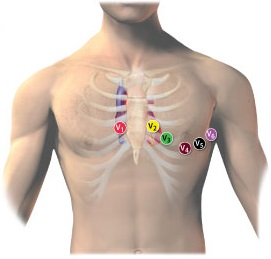
\includegraphics[width=.38\linewidth]{images/1311JEMSbg-12lead-p01.jpg}
%     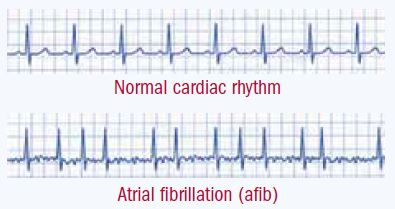
\includegraphics[width=.6\linewidth]{images/H1116-ECG.jpg}
%     \caption{Lead positioning in 12-lead ECG and atrial fibrillation event. Source: \href{https://www.jems.com/2013/11/07/12-lead-ecg-tips/}{Jems 2013} and \href{https://www.health.harvard.edu/heart-health/monitoring-your-heart-rhythm-with-a-smartphone-a-good-call}{Harvard Health Publishing}. Accessed in 12 October 2020.}
%     \label{fig:ecg_leads}
% \end{figure}

% O trabalho deve ser feito em até 3 páginas (formato livre). Todas as perguntas devem ser respondidas em até 3 páginas. Por favor, leia atentamente as instruções a seguir.
% 
% 1. Defina Ética em Inteligência Artificial. 
% 
% - A definição não precisa ser necessariamente com as suas palavras, mas precisa ser minimamente interpretada por vocês. Não basta copiar e colar a definição de alguém. 
% - Coloque a referência da definição. 
% 
% 2. Apresente e descreva uma notícia recente (de 2020) de um problema de Ética em IA. 
% 
% - Coloque a referência da notícia, ou seja, título da notícia, veículo de publicação, data da notícia, nome(s) da(s)/do(s) jornalista(s) e o link.
% 
% 3. Apresente um artigo científico recente (de 2020) de uma solução para um problema de Ética em IA. Descreva o problema e a técnica utilizada.
% 
% - Coloque a referência da artigo, ou seja, título do artigo, nome(s) da(s)/do(s) autora(e)(s), local de publicação (nome da conferência/workshop ou do periódico), data de publicação, número de citações do Google Acadêmico/Scholar (https://scholar.google.com/) e o link do artigo. 
% - Pode ser artigo (ainda não publicado) do arXiv.
% - O número de citações do Google Acadêmico/Scholar pode ser zero. Tudo bem.
% - Sugestões (mas, não apenas) de termos para procura de workshop/conferência/periódico: fairness, accountability, transparency, ethics. 
% 
% Observação: Para as três perguntas, as referências podem ser em português ou em inglês. Mas, possivelmente, encontraremos mais artigos científicos publicados na língua inglesa. 


% https://plato.stanford.edu/entries/ethics-ai/
% https://en.wikipedia.org/wiki/Ethics_of_artificial_intelligence]
% https://towardsdatascience.com/ethics-of-ai-a-comprehensive-primer-1bfd039124b0


\renewcommand{\refname}{References}
\bibliography{ref.bib}
\end{document}


